\section{Past breakthroughs}

\begin{frame}{Model initialization}
  \begin{figure}[H]
    \centering
    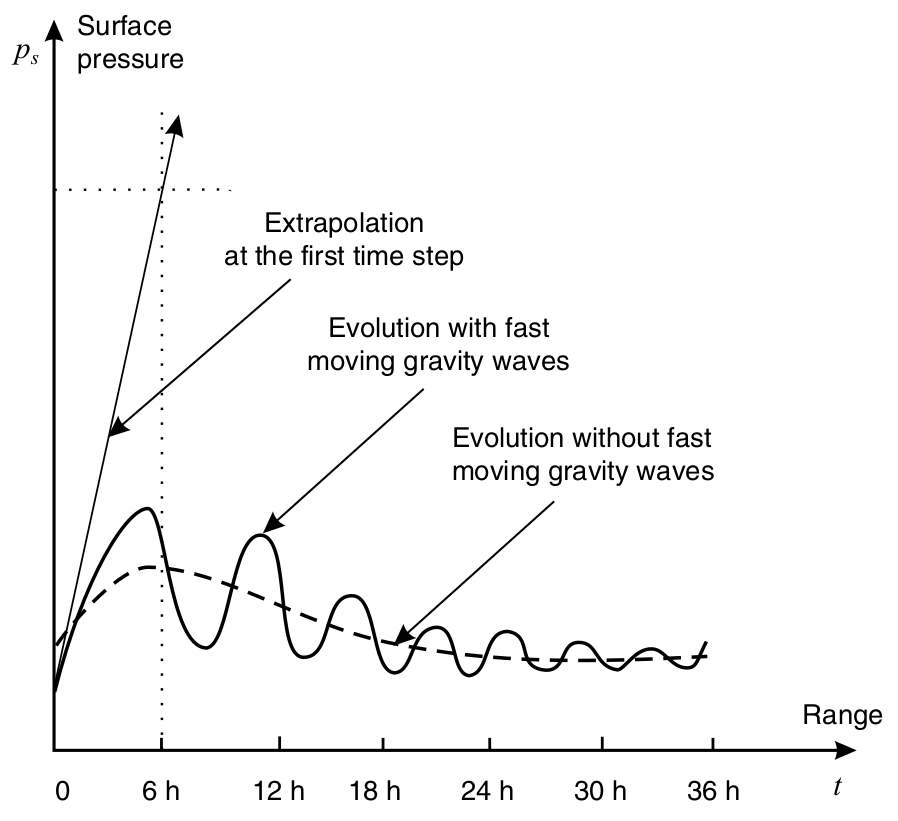
\includegraphics[width=0.6\textwidth]{../figures/nwp_pressure}

    \parencite{nwp}
  \end{figure}
\end{frame}


\note{
  Since forecasting is an initial value problem, crucial to know the state
  of the atmosphere.

  Evolution of surface pressure in:

  Model with fast moving gravity waves

  Without fast moving gravity waves

  Problem - Inital state not balanced -> oscillations due to gravity waves.
  Richardsons problem, since used full primitive equations


}

\begin{frame}{Model initialization}
  \begin{wideitemize}
    \item Synoptic analysis
    \item Objective analysis
    \item 3D / 4D variational data assimilation
  \end{wideitemize}
\end{frame}

\note{
  Forecasters takes the synoptic observations twice daily -> Visual interpolation on
  weather charts. Feeds into the computer.

  As the number of observations increased, performed by computers, objective analysis.

  Normal modes -> decompose atmospheric state into parts leading to
   Rossby waves,
   Eastward and westward gravity waves
   Only keep rossby mode

  Lynch and Huang 1992, shows this is equivalent to applying a low pass filter
  for the first 6 hours of a model run.

  3D / 4D variational methods includes a penalty term quantifying the lack of
  balance in a model.
}


\begin{frame}{Physical processes}
  \begin{figure}[H]
    \centering
    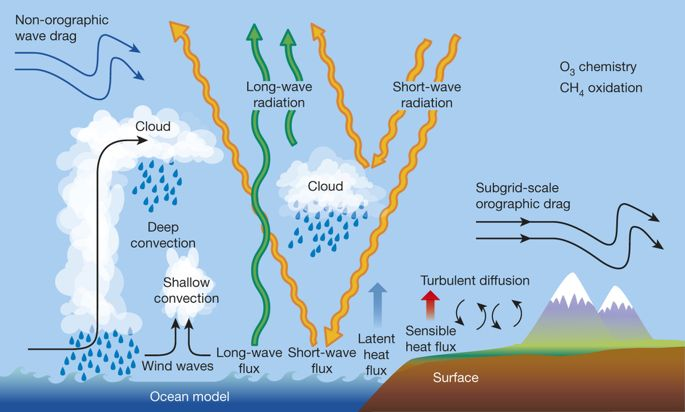
\includegraphics[width=0.8\textwidth]{../figures/bauer_physical.jpg}

    \parencite{bauer}
  \end{figure}

\end{frame}



\note{

Subgrid-scale prosseses can affect the  momentum, heat and water vapor buget at
grid scale.

Turbulence, condensation evaporation, friction, radiation.

\begin{wideitemize}
  \item Better understanding of the physical processes
  \item Grid scale invariance 10-100km
\end{wideitemize}

}


\begin{frame}{Ensemble}
  \begin{wideitemize}
    \item Probabilistic forecasting
    \item Poor mans ensemble
    \item Singular vector + Vector breeding
  \end{wideitemize}


  \begin{figure}[H]
    \centering
    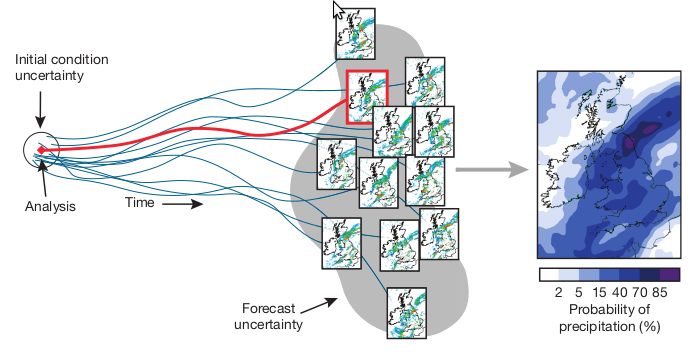
\includegraphics[width=0.6\textwidth]{../figures/nwp_ensemble.jpg}

    \parencite{nwp}
  \end{figure}


\end{frame}

\note{

  Since the results are so sensitive to the initial conditions, a move was made
  from deterministic to probabilistic forecasting.

  Several model runs (ECMWF runs 50) to calculate the probability

  Hard part of ensemble modelling - initial conditions that makes the output
  representative of the possibilities.

  Leith 1974 - Monte carlo method, small random perturbations to the initial state.
  Not sufficient.

  Rosseau and chapelet 1985 - Used the output of 7 different models. This was later
  proven not to be sufficient.


  Buizza 1993 -> Singular vector
  Useful on short time ranges (48h)
  Assume linearity in the error growth.
  Choose initial conditions that gives maximal growth in error.

}





\begin{frame}{Computational power}

  \begin{wideitemize}
    \item Model run time
    \item CFL-criteria
  \end{wideitemize}

  $$ T = \frac{N_v N_c N_t}{R}$$

  $$ \frac{U \Delta t}{\Delta x} < C $$

\end{frame}

\note{
Time used to run model

N$_v$ - number of variables.

basic variables to describe atmosphere * number of grid points

Number of grid points, surface of the earth / grid area.

N$_c$ - Calculations pr timestep - 10**3

N$_t$ - number of time steps

R - Calculation speed


C - factor dependent on geometry of grid.

U - fastest travelling wave. Decrease grid size -> smaller time step.

The last 70 years we have seen a doubling in computational power every 18 months.
Possible to run models with lower grid sizes.

}
